\chapter{Vector boson scattering in the standard model and beyond}
\label{ch:phenomenology}
The particle content of the SM was established over decades through
observations of radioactive decays, cosmic rays, and particle
collisions at accelerators, as discussed in Chapter~\ref{ch:introduction}. 
To the best of our
current knowledge, all collisions at the LHC involve only these objects,
interacting via the known forces.
However, there are tantalizing hints of additional particle content and the 
interactions based on cosmological observations, which suggest a ``dark matter''
that interacts gravitationally but not electromagnetically. In addition, 
the fact that the SM does not exclude additional particles or interactions at
higher energy scales is sufficient motivation to look for them. Due to the success
of the SM in describing our current set of observations, we expect these
``new physics'' modifications to respect our current observations.
This chapter introduces the mathematical formalism of the SM, and possible
extensions that are probed by the experimental results of this thesis.

\section{Mathematical formalism of the standard model}

Through these experimental tests and
discoveries, we have also built a description of all the known interactions 
of the SM particles in the language of gauge quantum field theory (QFT).
Particles in QFT arise as excitations in quantum fields.
The equations of motion and interactions for the quantum fields of the SM can
be extracted from the SM Lagrangian, which can be divided in to 
terms governing the propagation of free fields of the spin $1/2$ fermions,
the quarks and leptons, the spin 0 Higgs field, and the gauge fields:
\begin{equation}
  \mathcal{L}_{SM} = \mathcal{L}_{\text{gauge}} + \mathcal{L}_{\text{leptons}} + 
      \mathcal{L}_{\text{quarks}} + \mathcal{L}_{\text{scalar}} \,.
  \label{eq:smlagrangian}
\end{equation}
In this expression, $\mathcal{L}_{\text{gauge}}$ is a function of the 
spin 1 gauge fields---$G_a$, associated with the gluons of the strong
force, and $A_\mu$ and $\mathbf{b_{mu}}$, associated with the electroweak force.
The $\mathcal{L}_{\text{quark}}$ includes kinetic terms describing the 
propagation of free quarks as well as interaction terms coupling the quarks
to the gluon, $A_\mu$, and $\mathbf{b_\mu}$ fields. 
The term $\mathcal{L}_{\text{quarks}}$ is built from similar kinetic terms and 
interaction terms coupling the leptons to the electroweak fields, reflecting
the fact that the leptons do not participate in the strong interaction.

A fundamental property of the SM Lagrangian is its invariance 
under under so-called ``gauge transformations,'' in which a transformation 
of the fermion fields and the associated gauge field result in a mathematically
identical Lagrangian. The full SM Lagrangian respects transformations of the
group $\SUthree_C \bigotimes\SUtwo_L\bigotimes \Uone_Y$. 
In this expression, $\SUthree$ ($\SUtwo$) is the Lie group of all two-by-two
(three-by-three) matrices with determinant 1, and $\Uone$ is the Lie group
of complex numbers. The subscripts $C$, $L$, and $Y$ indicate the fermion
and gauge fields that are impacted by the rotation: the $\SUthree$ transformation
concerns only objects with color charge (quarks and gluons), and the $\SUtwo$
and $\Uone$ rotations concern weak isospin charge, which is carried only by 
the left-handed fermions, and weak hypercharge.

The measurements in this thesis are probe the structure of the gauge term
associated with the electroweak force. 

Follow the Quigg article to give some specifics for the EW force

\section{Electroweak symmetry breaking}

\section{Particle scattering and perturbative calculations}

Together with the principle of least action, the SM Lagrangian 
can be used to to derive the equations of motion of the SM fields. For the kinetic
terms, exact solutions can be obtained, however, closed-form equations of motion
do not exist when the interaction terms are also relevant.
The strength of these interaction is set by the coupling constants $g_i$
associated with the gauge fields, as described for the electroweak interaction
in Equations~\ref{}. If the couplings, and therefore the interactions, can be 
considered small, they can be treated as a perturbation of the free-field
propagation. Because field interactions are local, associated with 
a range of the interaction communicated by the gauge field,
this treatment is particularly well suited for scattering experiments.
Free, non-interacting fields are brought together in collision 
from a large separation, where the distance scale of the interacting fields
is proportional to the energy of the collision. After interaction,
free fields, possibly of different type than those brought to collision,
emanate from the interaction point.

\begin{figure}[htbp]
  \centering
   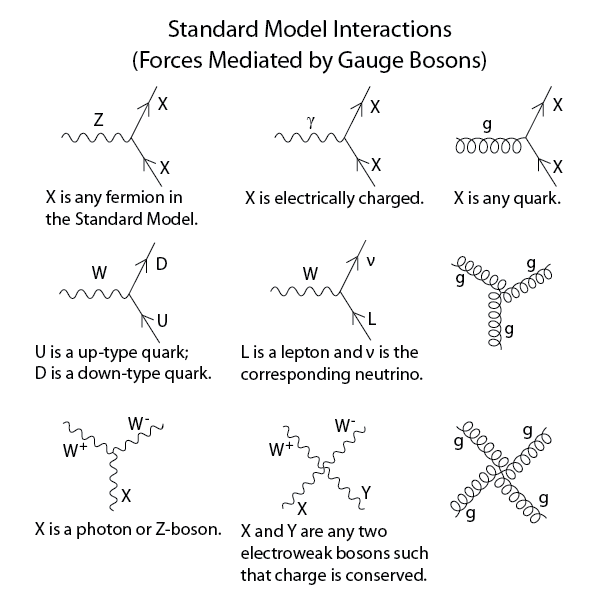
\includegraphics[width=0.6\textwidth]{figures/Phenomenology/Standard_Model_Feynman_Diagram_Vertices.png}
  \caption{
    Interactions allowed in the SM, excluding those involving the Higgs field.
        }
 \label{fig:SMinteractions}
\end{figure}

The allowed interactions in the SM are illustrated in Fig.~\ref{fig:SMinteractions}. Lines represent
propagating fields, and vertices represent interactions, arising from the
interaction terms in the SM Lagrangian. These illustrations,
known as Feynman diagrams, can be pieced together to give a diagrammatic
picture of a scattering interaction. Fig.~\ref{fig:wz3lfeynman} shows
an example quark-quark interaction---which contributions to $\pp$ collision
at the LHC---mediated by the $\PW$ and $\PZ$
bosons, leading to free muon, electron, and electron neutrino fields. 

\begin{figure}[htbp]
  \centering
   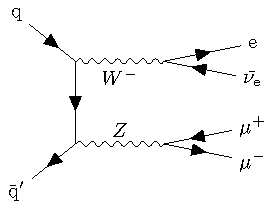
\includegraphics[width=0.4\textwidth]{figures/FeynmanDiagrams/WZ3lfeynman.pdf}
   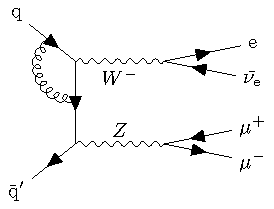
\includegraphics[width=0.4\textwidth]{figures/FeynmanDiagrams/WZ3lNLOfeynman.pdf}
  \caption{
    Feynman diagrams illustrating the $\Pq\Paq\to\mathrm{e}\PAGne\MM$ process,
    proceeding via quark and lepton couplings to the $\PW$ and $\PZ$ bosons.
        }
 \label{fig:wz3lfeynman}
\end{figure}

feynman diagrams are not just useful as an illustration, they 
represent terms in the perturbative expansion used to model
interactions.
They illustrate elements of the scattering matrix that 
connects the initial and final state in a scattering experiment. 
So-called Feynman rules
are used to associate the fields and interactions with the mathematical
formalism, giving mathematical expressions for the matrix elements
connecting the outgoing particle
four momenta and quantum numbers to the incoming particle properties.
Observables, including the total
rate of production for a final state given the initial state, are dependent
on the square of the scattering matrix elements.

The diagram in Fig.~\ref{fig:wz3lfeynman} (left) is not the only possible
set of interactions connecting the $\Pq\Paq$ initial state to the
$\mathrm{e}\PAGne\Paq\MM$ state. Other contributions include
diagrams where the $\PW$ and $\PZ$ bosons couple directly. In addition,
more intricate arrangements of the quark and gluon lines are possible,
as shown in Fig.~\ref{fig:wz3lfeynman} (right). A critical difference in
these two contributions to the $\Pq\Paq\to\mathrm{e}\PAGne\Paq\MM$ process is the
number of vertices, which contribute additional factors of the EW and
QCD couplings. If this coupling term is $\ll$1, the dominant contribution
will come from diagrams such as Fig.~\ref{fig:wz3lfeynman} (left), and
it may be possible to neglect the contribution of Fig.~\ref{fig:wz3lfeynman} (right).
Perturbative calculations rely on this approximation
by restricting a calculation to a maximum ``order'' $\mathcal{O}(\alpha^{n})$ 
in the coupling $\alpha \propto g^2$, by only considering
contributions to a process that have at most a dependence $\alpha^{n}$.

Depending on the process considered and the accuracy needed for a calculation,
neglecting the terms of ``higher order'' may not be appropriate. While the 
feynman rules are equally applicable for these terms, additional contributions
arise due to the presence of closed loops, as seen for the gluon and quark lines
in Fig.~\ref{fig:wz3lfeynman} (right). These individual diagrams give results
that predict infinite rates, therefore, they cannot correspond to experimental observations.
Fortunately, the situation can be recovered when combining with other diagrams
contributing to the higher-order calculation. A finite contribution can be
isolated and used to describe experimental measurements with incredible accuracy.
Infinite terms remain, but they can be associated with experimental-established
terms---in particular, the masses and couplings of the theory. This procedure,
known as renormalization, is closely connected to the energy scale of the process
and the structure fields themselves. In this approach, the coupling constant 
captures the neglected contributions from diagrams contributing at higher perturbative orders,
becoming an effective coupling at the energy scale considered.

\begin{figure}[htbp]
  \centering
   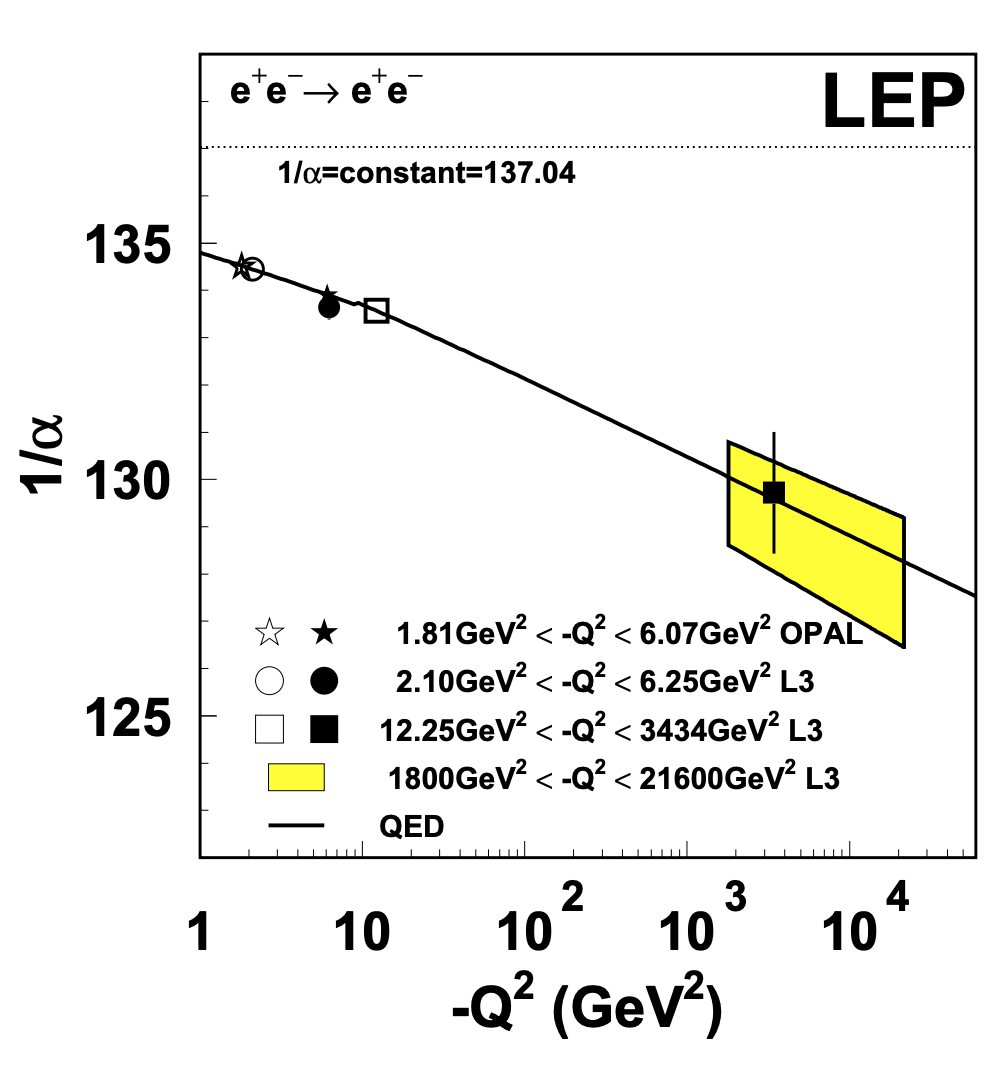
\includegraphics[width=0.39\textwidth]{figures/Phenomenology/alphaRunning.png}
   \raisebox{0.1\height}{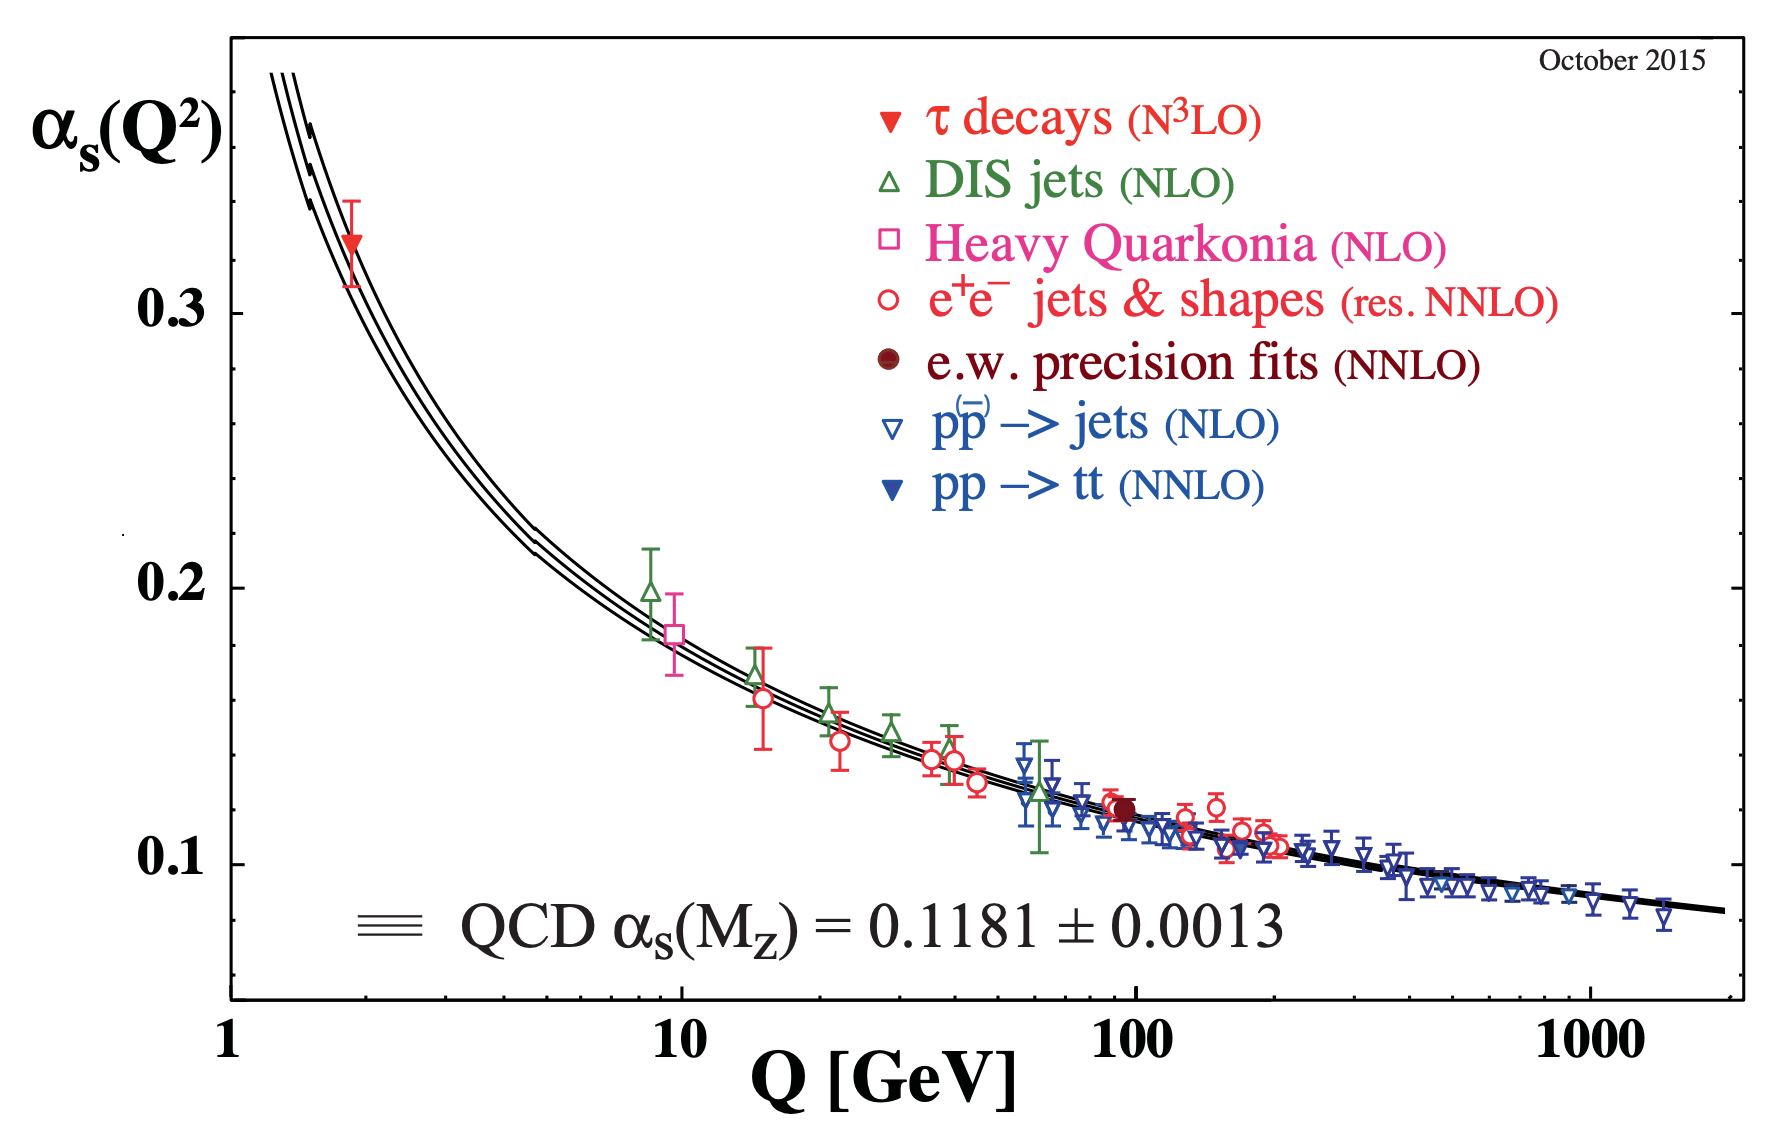
\includegraphics[width=0.59\textwidth]{figures/Phenomenology/alphasRunning.png}}
  \caption[The energy scale dependence of the effective EW and QCD couplings]{
    The energy scale dependence of the effective EW (left, reproduced from Ref.~\ref{Mele:2006ji}) 
    and QCD (right, reproduced from Ref.~\ref{Tanabashi:2018oca}) couplings. The theoretically
    predicted bands and discrete points established experimentally are shown.
  }
\end{figure}

The energy dependence of the effective coupling constants for the 
EW and QCD theories are shown in Fig.~\ref{fig:couplings}.
As shown, the nature of the $\SUthree$ and $\SUtwo$ forces leads to a striking difference
in energy dependence between the two theories: the EW coupling strength increases
with energy, whereas the QCD coupling decreases, leading to the 
confinement of quarks and gluons into bound states, such as the proton and neutron,
at low energies. At the energy scale probed in LHC collisions, the QCD coupling is
sufficiently small for perturbative calculations, however, higher-order corrections
are often significant. The scale dependence of the EW coupling is minimal, so
higher-order EW corrections are often not necessary
Perturbative calculations are discussed in more detail in Chapter~\ref{ch:simulation}.

\section{The \WZjj production at the LHC}
Here you need to build up the importance of multiboson production, and
how multibosons are produced at the LHC. First discuss WZ production,
then mention that ZZ has Higgs sensitivity.

Discuss multiboson prodution and its relevance to probing the EW sector
as well as calculations in quantum chromodyamics.

Discuss the WZjj QCD and EW components

\section{Probing the electroweak sector through vector boson scattering}

\section{New interactions in vector boson scattering}

Emboldened by the prospects of new physics in modifying \WZjj production
at the LHC, 

Introduction to the 


\subsection{Additional Higgs bosons and the Georgi-Machacek model}

In the SM, EWSB is realized by a single isospin doublet scalar field.
This field is sufficient to give mass to the $\PW$ and $\cPZ$
bosons, while resulting in the scalar $\PH$ boson, consistent with the observed
boson with $m_{\PH} = 125\GeV$.  Especially given the complexity of the fermion sector
of the SM, it is natural to ask if the universe contains a more complex
structure of scalar fields than the single doublet. 
However, SM extensions by arbitrary \SUtwo scalar fields 
are high constrained by the parameter $\rho \equiv m_\PW^2/m_\PZ^w\cos^2\theta$,
experimentally established to be very close to 1~\cite{}.
For a theory with $n$ scalar multiplets
$\phi_i$, with weak Isospin $I_i$, weak hypercharge $Y_i$, and vacuum expectation
value $v_i$, $\rho$ is given defined in terms of the quantum numbers of the fields
by the following expression at tree level~\cite{Branco:2011iw}
\begin{equation}
  \rho = \sum_{i = 1}^{n} \frac{I_i(I_i+1) - \frac{1}{4}Y_i^2}
              {\frac{1}{2}Y_i^2 v_i} \,,
  \label{eq:rho}
\end{equation}
Extending the scalar sector of the SM by two rather than one doublet satisfies
this expression. This model, known as the Two-Higgs-doublet model (2HDM), has
been extensively studied, in part because the scalar sector of SUSY has this form.
The 2HDM gives rise to a heavy Higgs boson, a pseudoscalar Higgs boson, and 
charged Higgs bosons $\PH^{\pm}$ in addition to a light SM-like Higgs boson.
In this model, the $\PH^{\pm}$ bosons coupling strongly to the leptons,
and decays to bosons are strongly suppressed in the mass range probed by the LHC~\cite{Arhrib:2016wpw}.

An alternative extension of the Higgs sector of the SM that satisfies experimental
constraints on $\rho$ was first proposed by Georgi and Machecek~\cite{Georgi:1985nv}.
In the Georgi Machacek (GM) model, the Higgs sector is extended by a real 
triplet with $Y=0$ and 
a complex triplet with $Y=2$ in addition to the usual SM doublet ($Y =1$). 
After EWSB, this leads to a rich Higgs sector with intriguing phenomenology.
The Higgs sector of the GM has ten physical states that are organized based
on their transformation properties under the approximate global $\SUtwo$ symmetry
of the scalar fields, referred to as custodial symmetry. There are two singlets,
one of which is associated with the observed Higgs boson, a triplet, and 
a fiveplet ($\PH_5^{++}$,$\PH_5^{+}$,$\PH_5^{0}$,$\PH_5^{-}$,$\PH_5^{--}$) that
is fermiophobic. If the mass of the triplet states is greater than the
mass of the fiveplet, the only production mechanism for $\PH^{\pm}$ at the LHC
is vector boson fusion. The production cross section is proportional to the variable
$s_{\PH}^2 \equiv \sin^2{\theta_{\PH}} = $, the ratio
of the vacuum expectation values of the triplet fields. Therefore, the leptonic $\WZjj$ 
state probed in this thesis is well-suited for further probes of this model, 
which is significantly less constrained than those charged Higgs with predominantly
leptonic decays.

\subsection{Generalizing new interactions with effective field theory}

If new physics is present VBS WZ production 

\section{Previous results}

\subsection{Measurements of \WZ production}

\subsection{}
